\documentclass[12pt, legalpaper]{article}

\usepackage[margin=3cm]{geometry}
\usepackage{natbib}
\bibliographystyle{unsrt} % or another style like unsrt, abbrv, etc.

\usepackage{algorithm}
\usepackage{algorithmic}

\usepackage{amsmath}
\usepackage{amssymb}

\usepackage{graphicx} % Required for inserting images
\usepackage{hyperref}
\usepackage{cleveref}

\usepackage{datetime}

\newdateformat{monthyeardate}{%
  \monthname[\THEMONTH], \THEYEAR}



  
\title{Automated algorithmic innovator MVP}
\author{The Innovation Game Labs}
\date{\monthyeardate\today}

\begin{document}

\maketitle





%%%
\section{Introduction}

Recent advances in LLM-powered coding have allowed LLMs to incorporate the coding ability into evolutionary processes for innovating entire algorithms given a target computational task, both at the conceptual and direct implementation level. 
In particular, Google DeepMind have released a line of research \citep{romera2024mathematical, novikov2025alphaevolve} where LLM-based systems are capable of finding novel algorithms beyond current human knowledge. 
This is both exciting and alarming for the future outlook of innovation and science, as such self-improving systems can lead to technological singularity that is controlled by a small number of centralised for-profit entities. 


%%%
\paragraph{Automating algorithmic improvements with LLMs}

LLMs have shown remarkable capability for code generation \citep{wang2023review, liu2023your} as well as mathematical understanding \citep{holt2024data, merler2024context}. 
Traditional evolutionary approaches to searching programs implementing algorithms typically involve manual specifications for intermediate code modifications that plug into the framework for genetic programming \citep{koza1994genetic, banzhaf1998genetic}. 
With LLMs, one can use prompt engineering to obtain valid program modifications and thus define transitions directly in the space of possible programs \citep{morris2024llm}. 
Evolutionary strategies that combine LLMs to search the space of functions have led to the discovery of novel mathematical results as shown in FunSearch \citep{romera2024mathematical, ellenberg2025generative}, and further applications have led to successful automation in the domain of science \citep{lu2024ai}, Bayesian optimisation \citep{aglietti2024funbo} and academic research idea generation \citep{li2024chain}. 
This idea has recently been generalised to searching directly over programs \citep{novikov2025alphaevolve} to evolve algorithms more flexibly given some target computational problem. 



%%%
\paragraph{Automating decentralised algorithmic innovation in TIG}

At The Innovation Game (TIG), our goal is to empower the open source community by creating a decentralised ecosystem for algorithmic innovation that leads to competitive algorithmic innovation with industry dominant closed source for-profit entities. 
In particular, the compute network accrued by TIG as well as the competitive open source nature of the reward incentives provides a decentralised alternative to the conventional privatised research labs that excel in the current AI landscape where massive compute is required for reaching state-of-the-art results. 
The rise of automated LLM-based algorithmic innovation machines has prompted us to build our own custom framework for automated algorithmic innovators that can eventually be plugged into the network of TIG alongside current human innovators. 
In this whitepaper, we present the technical foundations for our implementation of our baseline automated algorithmic innovator and directions for further development. 




%%%
\section{Automated algorithmic innovator MVP}



%%%
\subsection{High-level overview}\label{sec:highlevel}

We present a minimal implementation of the automated innovator that is very easily understood and yet capable of algorithmic improvement, while being highly customizable for adapting to more sophisticated evolution pipelines and prompt construction. 
This minimum viable product (MVP) will form the foundation for further research and development of the automated innovator within TIG. 


%
\paragraph{Goals}


At a high level, we design the MVP with the following goals in mind: 
%
\begin{itemize}
    \item Accessible to a wide audience of researchers and software engineers

    \item Highly customisable and easy to understand codebase for others to build on

    \item Exhibits basic ability for automated algorithmic innovation
\end{itemize}
%
Our pipeline is based on distilling key ideas from existing works like FunSearch \citep{romera2024mathematical} and AlphaEvolve \citep{novikov2025alphaevolve} into a simplified minimal pipeline with modular components for adding more sophisitication. 




%%%
\paragraph{Design}

To align with these goals, we design our MVP automated innovator pipeline in Python. 
The overall pipeline consists of a \emph{LLM} that generates code candidates and reasoning text, a code \emph{evaluator} that runs candidate algorithm programs and a collection of \emph{prompts} constructed based on the target computational problem and valid algorithm input and output structure: 
%
\begin{itemize}
    \item The user specifies the computational problem to be solved, the evaluation metrics the \emph{LLM} will receive from the \emph{evaluator} and the target metric to improve upon. These will be combined into a \emph{system prompt} which conditions the \emph{LLM} to a desired personality and response structure for our framework structure, which requires the \emph{LLM} to output a separate \emph{code} block and \emph{reasoning} comments

    \item The user provides a sample algorithm code implementation that contains basic comments to outline the algorithm process. Note this code sample does not have to be a valid program and can in fact even be a code skeleton outline, as the pipeline will automatically attempt to correct invalid program submissions

    \item Finally, the user also specifies the \emph{evaluator} backbone code that imports the algorithm implementation from the program submissions as a Python function that can be used inside a standardised evaluation pipeline. This is similar to FunSearch \citep{romera2024mathematical}, but we allow complete freedom in the modification of the algorithm function like AlphaEvolve \citep{novikov2025alphaevolve}
\end{itemize}
%
These components make up the following evolution pipeline: 
%
\begin{enumerate}
    \item The proposed program \emph{code} (provided in the first step, generated after) is fed into the \emph{evaluator} components for execution on a fixed set of problem instances as done in FunSearch \citep{romera2024mathematical}. In case of invalid \emph{code}, the \emph{evaluator} will return the Python interpreter error traceback instead of evaluation metrics

    \item The \emph{evaluator} feedback results and \emph{reasoning} comments for writing this code (none in the first step) are concatenated with the program \emph{code} into the next prompt for sending to the \emph{LLM}

    \item The \emph{LLM} response is checked for valid output structure so that the \emph{code} and \emph{reasoning} blocks can be extracted and stored. In case of invalid structure, we resend the prompt with a indication of invalid output response attached to it, and keep repeating this until a valid response is generated

    \item We go back to step 1 with the new \emph{code} and \emph{reasoning} blocks while appending all intermediate output components to the evolution chain storage, and stop if we reached the maximum number of evolution steps
\end{enumerate}
%
The overall evolution structure forms a simple linear chain as shown in \autoref{fig:schematic}, without any branching or mixing between individual chains. 
This is a significant simplification compared to the island-based evolution structure used in FunSearch and AlphaEvolve \citep{romera2024mathematical, novikov2025alphaevolve}, which use a dedicated program database and sampling schemes to construct new prompts. 
In contrast, our linear evolution chain gives direct access to the previous proposed program with its evaluation performance, and allows storing results and knowledge from the deeper past inside \emph{reasoning} responses. 
The code implementation of this pipeline is available on our public GitHub repository\footnote{\url{https://github.com/tig-foundation/automated-ai-innovator}}. 






%%%
\subsection{Target computational problems}\label{sec:comptasks}


\begin{figure}[t]
    \centering
    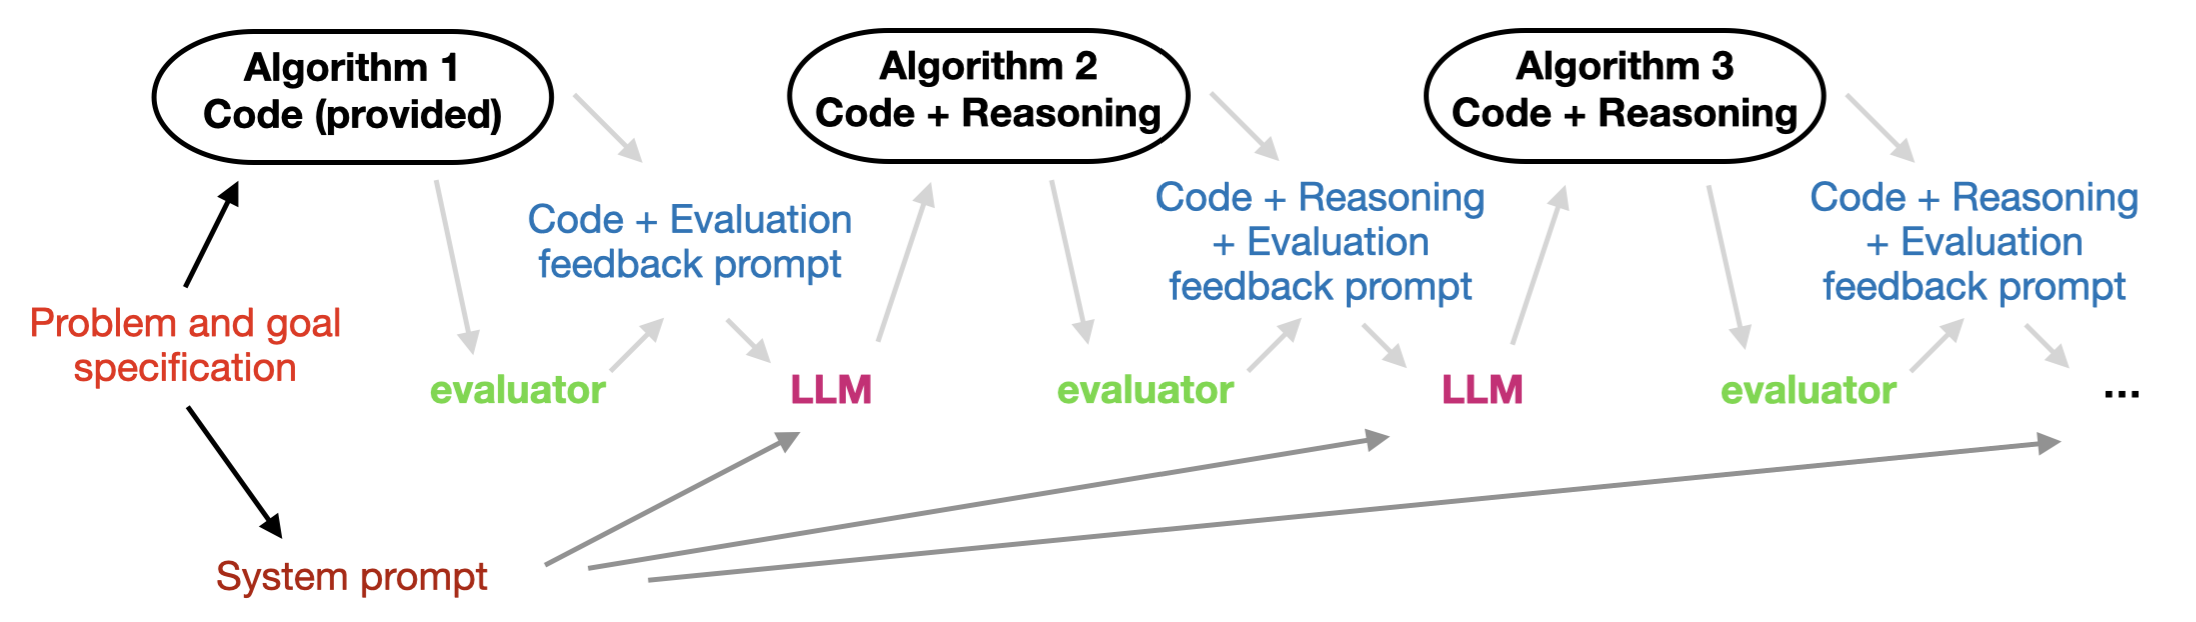
\includegraphics[width=\textwidth]{figures/schematic.png}
    \caption{
    \textbf{Schematic of the automated algorithmic innovator MVP.} 
    The pipeline as described in \autoref{sec:highlevel} is shown here as a flowchart, with separate components individually coloured. 
    Note the linear evolution chain structure, which is the simplest structure for running a self-improving agent that uses its own past proposal and evaluation feedback. 
    }
    \label{fig:schematic}
\end{figure}

Given our basic functionality, we test our MVP on prototype TIG "mini-challenges", which are designed to be simple computational problems that have a qualitatively similar computational asymmetry aspect (hard to improve, easy to verify) to real TIG challenges. 
These mini-challenges are constructed with the following principles in mind: 
%
\begin{itemize}
    \item Easy to understand intuitively with minimal background knowledge
    
    \item Easy to visualize the computational problem and candidate solutions
    
    \item Relies heavily on heuristics, often with human-interpretable justification, allowing one to create interpretable reasoning chains for algorithm improvements
    
    \item Has good room for algorithmic improvement and innovation to showcase algorithmic innovation ability without sophisticated and compute-heavy pipelines
\end{itemize}
%
We propose and implement the following mini-challenges:

\paragraph{Kernel Density Estimation (KDE)}

In this task, the goal is to construct a Gaussian mixture model (GMM) that describes the underlying density of a set of points $\mathbf{x} \in \mathrm{R}^D$ sampled from a non-injective nonlinear transformation of a unit Gaussian random variable. 
This transformation is implemented with a randomly initialised multi-layer perceptron (MLP) using rectified linear activation functions \citep{rosenblatt_perceptron_1958}, and thus the ground truth density $p(\mathbf{x})$ is intractible. 
We sample training $\mathbf{x}_{\text{train}} \sim p(\mathbf{x})$ and test $\mathbf{x}_{\text{test}} \sim p(\mathbf{x})$ sets, and the evaluation metric to maximize is the test log likelihood of the test set points using the GMM constructed with the training set points. 
Due to $p(\mathbf{x})$ being intractable, finding the best GMM is an asymmetric problem. 
Valid algorithms take as input the training set $\{ \mathbf{x}_{\text{train}} \}$ and output GMM means $\in \mathrm{R}^D$ and covariances $\in \mathrm{R}^{D \times D}$, with a freedom to choose the number of mixture components. 
Covariances that are not positive definite will lead to an error in the evaluator pipeline. 
Heuristics for finding good GMM parameters have become textbook standard \citep{Silverman1986}. 




\paragraph{Clustering}


Here, the goal is to group a set of points $\mathbf{x} \in \mathrm{R}^D$ by assigning each point to one of the $K$ clusters, where $K$ is fixed as part of the problem specification. 
The points are sampled from a similar transformation as in KDE, but we do not split between training and test set as the evaluation metric for clustering is computed on the set of points clustering was performed over. 
In particular, we use a pairwise connectivity-based clustering score 
%
\begin{equation}
    \sum_{i=1}^{n} \sum_{j \in \mathcal{N}_i} \frac{1}{\text{rank}_{ij}} \cdot \mathrm{1}_{c_i \ne c_j}
\end{equation}
%
Valid algorithms take as input the set of points $\{ \mathbf{x} \}_i$ and output cluster identities $c_i \in \{1, 2, \ldots, K \}$ per point. 


\paragraph{Histogram Density Estimation}

Similar to KDE, we now perform density estimation but instead of using a GMM we use piecewise constant probability density candidates (histograms with potentially non-uniform binning). 
As histograms suffer from the curse of dimensionality, we restrict ourselves to $D=1$. 
In addition, we restrict the points to a finite range $x \in [-1, 1]$ which is achieved by replacing the activation function in the MLP with a sinusoid \citep{sitzmann2020implicit}, including the final layer. 
Valid algorithms take as input the training set $\{ x_{\text{train}} \}$ and output bin boundaries within the $[-1, 1]$ interval, with boundaries placed at $\pm 1$ by default. 
The algorithm has the freedom to decide the number of bins to use. 


%%%
\section{Preliminary results}


\begin{figure}[t]
    \centering
    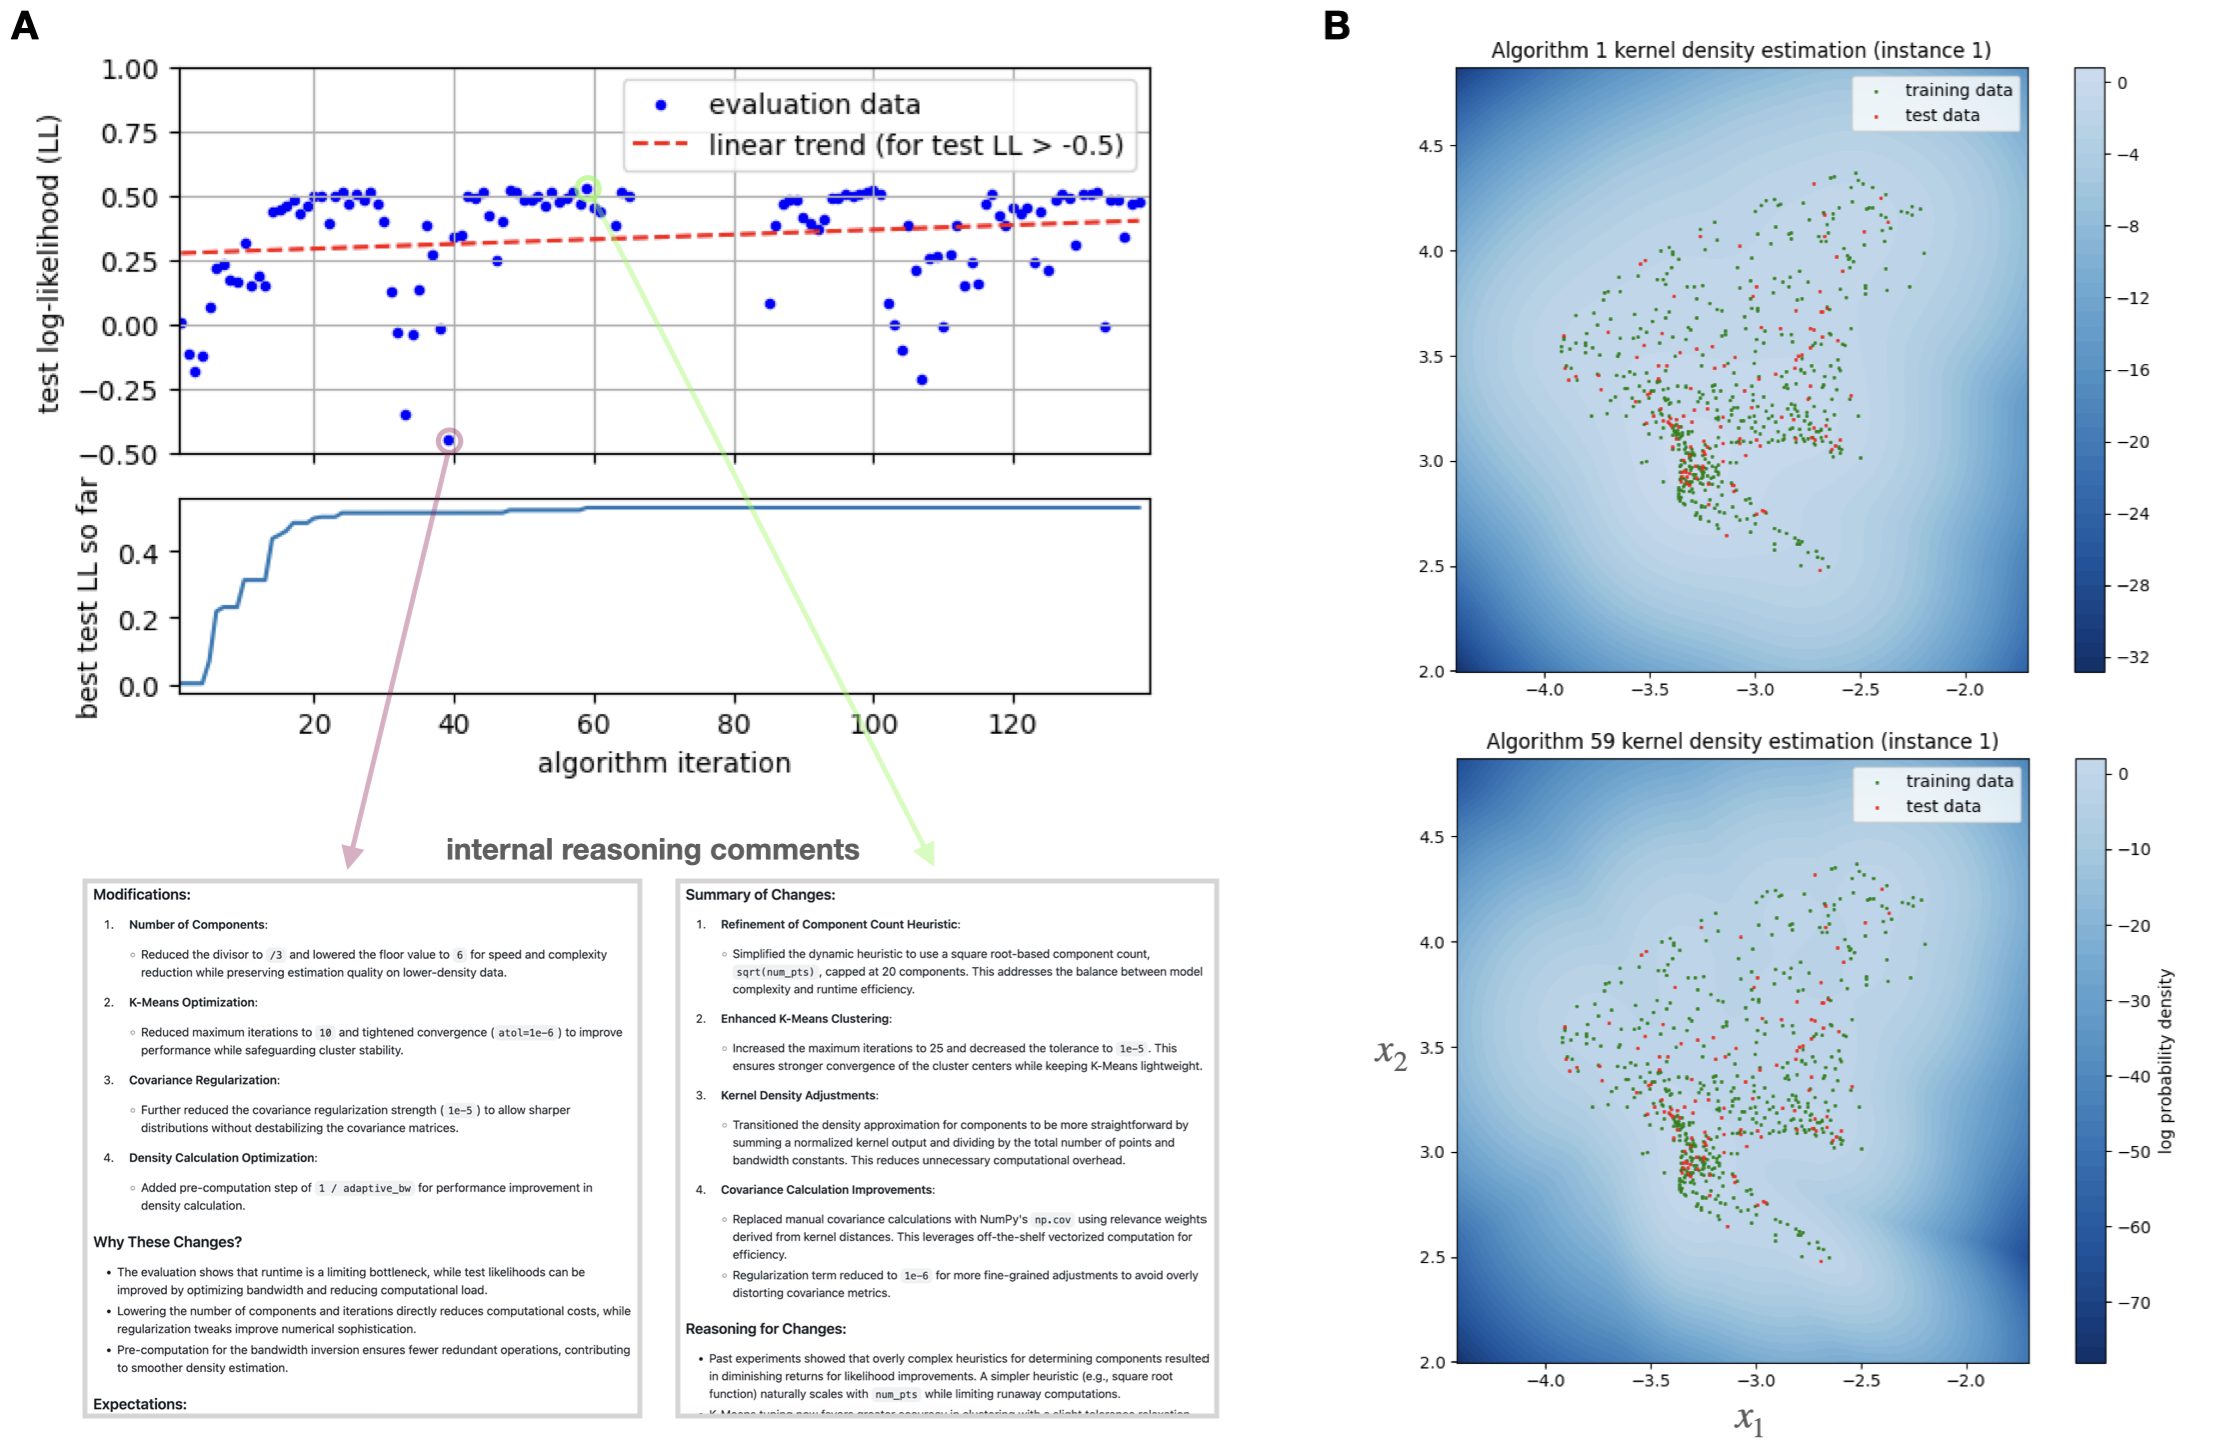
\includegraphics[width=\textwidth]{figures/challenge_KDE.png}
    \caption{
    \textbf{Example evolution run with the KDE problem with $D=2$.} 
    \textbf{(A)} Performance plot of a successful evolution chain (top). 
    Invalid programs resulting in NaN scores, which show up as missing entries in the scatter plot. 
    In addition, the LLM occasionally generates bad outlier programs that lead to very low test LLs, which are not plotted and considered in the linear trend fit (red dotted line) for keeping the visualisation clear. 
    The best performing algorithm was at index 59, and we show example internal reasoning comments along the evolution process (bottom). 
    \textbf{(B)} Visualising the log probability density estimated from algorithm 1 (top) and algorithm 59 (bottom). 
    }
    \label{fig:challenge_KDE}
\end{figure}


We show a successful sample run on the KDE mini-challenge in \autoref{fig:challenge_KDE}, where the pipeline discovered a better KDE algorithm using $k$-means clustering compared to the seed algorithm implementing Silverman's rule of thumb \citep{Silverman1986}. 
Our pipeline uses the internal reasoning comments (acting as a recurrent hidden state as shown in \autoref{fig:schematic}) to justify and keep track of code changes. 
Using prompt and program evaluation history has been shown to improve evolution performance significantly \citep{novikov2025alphaevolve}, and in our pipeline the reasoning pattern forms a simple linear chain that can be visualised and studied. 
The structure of the reasoning comments is not currently specified in the system prompt, and is designed by the LLM autonomously. 
Note that many evolution runs typically fail to improve or get stuck in a suboptimal minimum, given the combinatorial complexity of the optimisation problem, which justifies the use of more complicated evolution dynamics and structures such as multi-population and island-based structures \citep{romera2024mathematical, novikov2025alphaevolve}. 



%%%
\section{Discussion and further work}\label{sec:further}

We presented a MVP for the automated algorithmic innovator in the context of TIG. 
The minimalist and modular pipeline design allows one to easily expand the capabilities with various approaches to introduce more sophistication. 


\paragraph{More sophisticated evolution pipelines}

Due to the combinatorial complexity of optimising directly in the space of all valid programs, our simple linear evolution chain is limited in the sample efficiency it can achieve. 
Many techniques from this field like cross-overs between independent evolution chains, genetic programming and island-based structures are used in state-of-the-art frameworks like FunSearch and AlphaEvolve \citep{romera2024mathematical, novikov2025alphaevolve}. 
The simplest extensions to our pipeline are for example:
%
\begin{itemize}
    \item Incorporating a program database instead of storing all past dependence in the most recent reasoning comment and the context of the LLM

    \item Introducing a cross-over mechanism between parallel evolution chains to reset runs that are stuck in bad optima
\end{itemize} 
%
Several open source implementations of more sophisticated evolution frameworks for algorithm optimisation are available, like open source AlphaEvolve repositories aiming to reproduce the original publication (\href{https://github.com/codelion/openevolve}{https://github.com/codelion/openevolve} and \href{https://github.com/shyamsaktawat/OpenAlpha_Evolve}{https://github.com/shyamsaktawat/OpenAlpha\_Evolve}), as well as related self-evolving coding agent frameworks like \href{https://github.com/jennyzzt/dgm}{https://github.com/jennyzzt/dgm}.


\paragraph{Fine-tuning LLMs for algorithmic innovation}

Training LLMs is a costly project \citep{nikolic_survey_2022}, and to obtain LLMs improved for specific tasks like conversation or algorithmic design, massive training costs can be avoided by fine-tune trained base LLMs. 
These techniques are referred to as "post-training" since they are applied after the expensive "pre-training" of the base LLMs on a large general corpus. 
There are various approaches to fine-tuning, including supervised approaches \citep{stiennon2020learning}, reinforcement learning (RL) using a reward model trained on human preferences \citep{ouyang2022training, ye2025robust}, and more recently even self-supervised techniques \citep{wen2025unsupervised}. 
Notably, DeepSeek-R1 \citep{guo2025deepseek} has shown that it is possible to get rid of the expensive critic neural network typically required in policy gradient methods like PPO \citep{schulman2017proximal} used to fine-tune LLMs with RL. 
By grouping multiple responses of the LLM to the same prompt and using the group average as a reward baseline, a stable learning signal can be obtained at a much lower cost. 
Furthermore, by rewarding coding and mathematics related Chain-of-Thought (CoT) paths that lead to executable and provably correct results, the fine-tuning process is able to elicit better coding and mathematical reasoning properties from the base LLM. 
In our pipeline, we can regard reasoning chains from evolution runs with their metric scores as data points for RL to fine-tune LLMs for improvement \emph{algorithmic innovation} abilities across various computational problems. 


\paragraph{Incorporating RL-swarms for fine-tuning}

Gensyn's RL-swarm\footnote{\url{https://github.com/gensyn-ai/paper-rl-swarm}} extends DeepSeek-R1's group-based approach to fine-tuning multiple LLMs simultaneously, allowing one to construct a group with LLM responses from multiple LLM peers. 
This new paradigm touches upon multi-agent RL, and they report improved training performance from preliminary results due to added exploration from LLM peers inside groups. 
The RL-swarm framework can be naturally combined with our automated innovator in a network setting, where individual innovator nodes may deploy different LLMs and can collaborate with each other by forming a RL-swarm to improve fine-tuning of their LLMs jointly. 


\paragraph{Multi-agent framework}

In our MVP, we rely on a single LLM that handles all the code modifications and reasoning for algorithmic innovation. 
One can dissect the overall code improvement process into separate parts, such as code suggestions and reasoning chain formation, and assign separate LLMs to each. 
This moves to the multi-agent approach, which has been applied to various practical scientific research problems such as bridging knowledge gaps across expert domains \citep{aryal2024leveraging}. 




\bibliography{references} % references.bib is the file containing the bib entries

\end{document}